% !TeX spellcheck = cs_CZ
{\tikzset{external/prefix={tikz/FYZI/}}
 \tikzset{external/figure name/.add={ch33_}{}}
%=========================== Kapitola: Polarizace =================================================
\chapter{Polarizace}\label{fyz:IchapXXXIII}
\minitoc
  \section{Elektrický vektor světla}\label{fyz:IchapXXXIIIsecI}
  \section{Polarizace rozptýleného světla}\label{fyz:IchapXXXIIIsecII}
  \section{Dvojlom}\label{fyz:IchapXXXIIIsecIII}
  \section{Polarizátory}\label{fyz:IchapXXXIIIsecIV}
  \section{Optická aktivita}\label{fyz:IchapXXXIIIsecV}
  \section{Intenzita odraženého světla}\label{fyz:IchapXXXIIIsecVI}
  \section{Anomální lom světla}\label{fyz:IchapXXXIIIsecVIII}
  \section{Příklady a cvičení}\label{fyz:IchapXXXIIIsecIX}

    \begin{figure}[ht!]  %\ref{fyz:fig270}
      \centering
      \begin{tabular}{ccc}
        \subfloat[ ]{\label{fyz:fig270a}
          \includegraphics[width=0.28\linewidth]{fyz_fig270a.pdf}}               &
        \subfloat[ ]{\label{fyz:fig270b}
          \includegraphics[width=0.16\linewidth]{fyz_fig270b.pdf}}               &
        \subfloat[ ]{\label{fyz:fig270c}
          \includegraphics[width=0.28\linewidth]{fyz_fig270c.pdf}}               \\
        \subfloat[ ]{\label{fyz:fig270d}
          \includegraphics[width=0.28\linewidth]{fyz_fig270d.pdf}}               &
        \subfloat[ ]{\label{fyz:fig270e}
          \includegraphics[width=0.28\linewidth]{fyz_fig270e.pdf}}               &
        \subfloat[ ]{\label{fyz:fig270f}
          \includegraphics[width=0.28\linewidth]{fyz_fig270f.pdf}}               
      \end{tabular}
      \caption{Skládání kmitů ve směru os \(x\) a \(y\) ve fázi
               (\cite[s.~437]{Feynman01})}
      \label{fyz:fig270}
    \end{figure}

    \begin{figure*}  %\ref{fyz:fig271}
      \centering
      \begin{tabular}{ccc}
        \subfloat[ ]{\label{fyz:fig271a}
          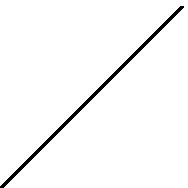
\includegraphics[width=0.2\linewidth]{fyz_fig271a.pdf}}               &
        \subfloat[ ]{\label{fyz:fig271b}
          \includegraphics[width=0.2\linewidth]{fyz_fig271b.pdf}}               &
        \subfloat[ ]{\label{fyz:fig271c}
          \includegraphics[width=0.2\linewidth]{fyz_fig271c.pdf}}               \\
        \subfloat[ ]{\label{fyz:fig271d}
          \includegraphics[width=0.2\linewidth]{fyz_fig271d.pdf}}               &
        \subfloat[ ]{\label{fyz:fig271e}
          \includegraphics[width=0.2\linewidth]{fyz_fig271e.pdf}}               &
        \subfloat[ ]{\label{fyz:fig271f}
          \includegraphics[width=0.2\linewidth]{fyz_fig271f.pdf}}               \\
        \subfloat[ ]{\label{fyz:fig271g}
          \includegraphics[width=0.2\linewidth]{fyz_fig271g.pdf}}               &
        \subfloat[ ]{\label{fyz:fig271h}
          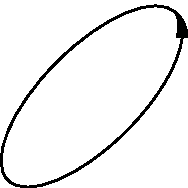
\includegraphics[width=0.2\linewidth]{fyz_fig271h.pdf}}               &
        \subfloat[ ]{\label{fyz:fig271i}
          \includegraphics[width=0.2\linewidth]{fyz_fig271i.pdf}}               
      \end{tabular}
      \caption{Skládání kmitů ve směru os \(x\) a \(y\) se stejnými amplitudami, 
               ale s různými relativními fázemi. Složky \(E_X\) a \(E_y\) jsou 
               vyjádřeny v reálném i komplexním tvaru
               (\cite[s.~437]{Feynman01})}
      \label{fyz:fig271}
    \end{figure*}
    
    \begin{figure}[ht!] %\ref{fyz:fig272}
      \centering
      \includegraphics[width=0.7\linewidth]{fyz_fig272.pdf}
      \caption{ 
               (\cite[s.~427]{Feynman01})}
      \label{fyz:fig272}
    \end{figure}

    \begin{figure}[ht!] %\ref{fyz:fig273}
      \centering
      \includegraphics[width=0.7\linewidth]{fyz_fig273.pdf}
      \caption{ 
               (\cite[s.~427]{Feynman01})}
      \label{fyz:fig273}
    \end{figure}

    \begin{figure}[ht!] %\ref{fyz:fig274}
      \centering
      \includegraphics[width=0.7\linewidth]{fyz_fig274.pdf}
      \caption{ 
               (\cite[s.~427]{Feynman01})}
      \label{fyz:fig274}
    \end{figure}

    \begin{figure}[ht!]  %\ref{fyz:fig275}
      \centering
      \begin{tabular}{cc}
        \subfloat[ ]{\label{fyz:fig275a}
          \includegraphics[width=0.28\linewidth]{fyz_fig275a.pdf}}               &
        \subfloat[ ]{\label{fyz:fig275b}
          \includegraphics[width=0.28\linewidth]{fyz_fig275b.pdf}}               \\
      \end{tabular}
      \caption{
               (\cite[s.~437]{Feynman01})}
      \label{fyz:fig275}
    \end{figure}

    \begin{figure}[ht!]  %\ref{fyz:fig276}
      \centering
      \begin{tabular}{cc}
        \subfloat[ ]{\label{fyz:fig276a}
          \includegraphics[width=0.28\linewidth]{fyz_fig276a.pdf}}               &
        \subfloat[ ]{\label{fyz:fig276b}
          \includegraphics[width=0.28\linewidth]{fyz_fig276b.pdf}}               \\
      \end{tabular}
      \caption{
               (\cite[s.~437]{Feynman01})}
      \label{fyz:fig276}
    \end{figure}


    \begin{figure}[ht!] %\ref{fyz:fig277}
      \centering
      \includegraphics[width=0.7\linewidth]{fyz_fig277.pdf}
      \caption{ 
               (\cite[s.~427]{Feynman01})}
      \label{fyz:fig277}
    \end{figure}

    \begin{figure}[ht!] %\ref{fyz:fig278}
      \centering
      \includegraphics[width=0.7\linewidth]{fyz_fig278.pdf}
      \caption{ 
               (\cite[s.~427]{Feynman01})}
      \label{fyz:fig278}
    \end{figure}

} %tikzset
%---------------------------------------------------------------------------------------------------
\printbibliography[title={Seznam literatury}, heading=subbibliography]
\addcontentsline{toc}{section}{Seznam literatury}